\documentclass[xcolor=dvipsnames,hyperref={pdfpagelabels=false}]{beamer}

\usetheme{Boadilla}

\newcommand{\bi}{\begin{itemize}}
\newcommand{\ei}{\end{itemize}}
\newcommand{\be}{\begin{enumerate}}
\newcommand{\ee}{\end{enumerate}}
\newcommand{\bc}{\begin{center}}
\newcommand{\ec}{\end{center}}
\newcommand{\bd}{\begin{description}}
\newcommand{\ed}{\end{description}}
\newcommand{\I}{\item}
\newcommand{\f}{\frame}
\newcommand{\ft}{\frametitle}

\title{What I Just Learned about TDCs}
\author[Mark Ito]{Mark M.\ Ito}
\date{November 19, 2014}
\institute[JLab]{Jefferson Lab}

\begin{document}

\f{\titlepage}

\f{\ft{The Timing Systems and Their System Clocks}
\begin{tabular}{|l|c|c|l|}
\hline
{\bf System} & {\bf Freq. (MHz)} & {\bf Period (ns)} & {\bf Use} \\
\hline
Flash-250 ADC & 250 & 4 & non-drift chamber \\
Flash-125 ADC & 125 & 8 & drift chamber \\
CAEN 1290 TDC & 41.67 & 24 & TOF \\
F1-TDC & 31.25 & 32 & not CDC, not TOF \\
\hline
\end{tabular}
\bi
\I The 250 MHz clock is special: it runs the trigger.
\I All clocks are ``synched'': the edges of any system clock have a fixed phase relation to all others.
\I Problem: times in each system need to reference their clock, different clocks imply different references (for F1-TDC it is worse). 
\I It suffices to put a single, fanned-out pulse into a signal channel of each system.
  \bi
  \I Needs to be there every event.
  \I RF time is a popular choice: ties time-scale to beam-on-target.
  \I Other choices bring systems into registration with each other. In this case, signal need not even be ``synched''.
  \I One channel per system suffices.
  \ei
\ei
}

\f{\ft{End of Story, Right?}
\bi
\I We will put such a signal in.
  \bi
  \I RF signal when we get it
  \I Trigger signal until we do
  \ei
\I We will rely on it
\I No need to go any further.
\I (laptops start opening at this point in talk)
\I Except...
\ei
}

\f{\ft{Why Try to Understand Things Further?}
\bi
\I We started running with no reference signal.
\I We have put trigger signals in but have not seen them in the data yet.
\I We have not demonstrated success in their use.
\I Timing plots in monitoring histograms have presented ``mysteries'' due to lack of understanding of system features.
\ei

Understanding how the timing systems work will:

\bi
\I Allow us to make sense of non-referenced, raw times.
\I Allow us to align timing systems without a reference signal.
  \bi
  \I Gives an independent check on the reference signal method.
  \I Demonstrates correct functioning of sub-groups of devices that may not have the reference signal.
  \ei
\I Allow us to hold our heads high as experimentalists.
\I Will not address intrinsic ``4 ns uncertainty.''
\ei
}

\f{\ft{CAEN 1290 TDC I}
\bi
\I Features
  \bi
  \I system clock period: 24 ns
  \I trigger signal comes into front-panel input(?)
  \I nothing happens until the next 24-ns-system-clock tick
  \I digitization is referenced to that clock tick
  \I works well for colliders where system clock edges = bunch crossing times
  \ei
\I Key System Feature
  \bi
  \I TI counts 4-ns clock cycles
  \I Counter reset at synch time (beginning of run)
  \ei
\ei
}
\f{\ft{CAEN 1290 TDC II}
$$
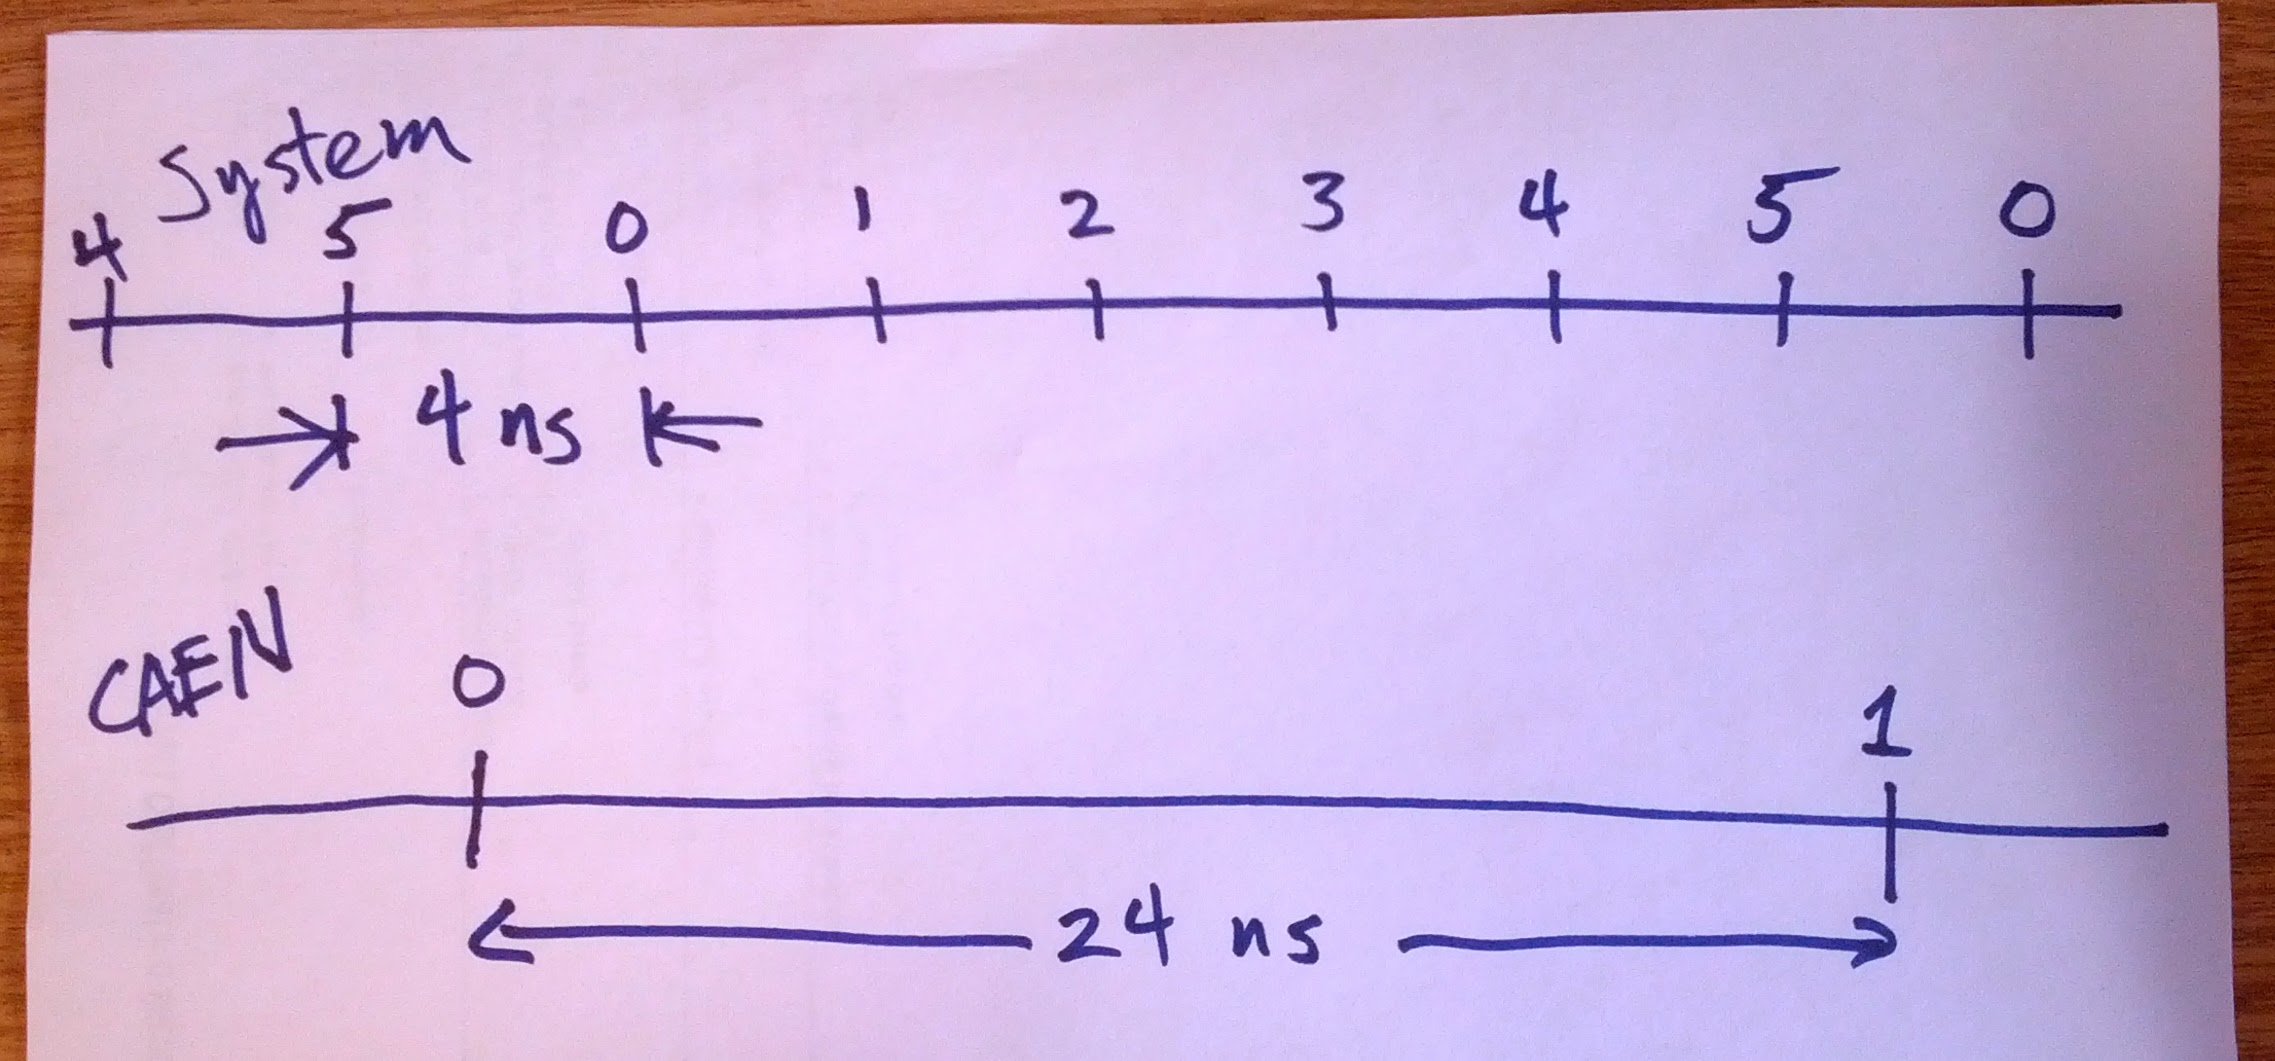
\includegraphics[height=1.8in]{timing_diagram.jpg}
$$
\bi
\I Problem
  \bi
  \I a 24-ns clock has a 6-fold phase ambiguity with respect to a 4-ns clock
  \I when trigger arrives time uncertain, with this ambiguity
  \ei
\ei
}

\f{\ft{CAEN 1290 TDC III}
\bi
\I Solution
  \be
  \I Make sure TI uses 48-bits for its counter (13 day wrap-around time)
  \I At synch time ``resynch'' the 24-ns clock with the 4-ns clock.
    \bi
    \I Requires firmware change in the TS.
    \I William Gu has already coded this up.
    \I Not yet installed in Hall
    \ei
  \I Use TI counter to measure the 6-fold phase ambiguity (TI counter modulo 6) 
  \ee
\ei
}

\f{\ft{F1-TDC I}
\bi
\I Features
  \bi
  \I F1 TDC codes run from a bit more than 0 to a bit less than $(2^{16} - 1) = 65535$, e.~g. 10 to 65525.
  \I ``Reset'' is when the code flips from the highest possible value to the lowest possible value (e. g., from 65525 to 10).
  \I There is a system clock going on a 32 ns period (31.25 MHz) all internal clock are derived from this one. A trigger time stamp is also generated with a 32 ns period starts at 0 and is read-out.
  \I For a 56 ps least count, the time between resets would be 3.67 microseconds if the count range were $2^{16}$ (which it is not).
  \I The trigger defines the beginning of the read-out window. The data values are completely insensitive to the details of window setting.
  \I The trigger time stamp is recorded from the TI
  \I The read-out window cannot be more than 90\% of the reset period, otherwise time differences would be ambiguous.
  \ei
\ei
}

\f{\ft{F1-TDC II}
\bi
\I Problem
  \bi
  \I Since the reset period is not a integral multiple of any clock period, it cannot be referenced to any internal time except for the initial reset at the beginning of the run.
  \I The initial reset happens on an edge of the 32-ns clock. The sync comes a 8-fold ambiguous time with respect to that clock.
  \ei
\I Solution
  \bi
  \I Re-synch TDC system clock at synch time.
    \bi
    \I Also part of William's firmware upgrade for TS.
    \ei
  \I Can reference time to the trigger by calculating trigger time using the TI counter.
    \bi
    \I Calculate number of reset cycles since synch (integer and fraction) from TI counter.
    \I Fractional part gives the corresponding TDC code.
    \I Treat this as the trigger time, as if it came from an input channel.
    \ei
  \I Then all codes in the system could reference this trigger time.
  \I This has never been attempted.
  \ei
\ei
}

\f{\ft{Flash-125 ADCs}
Have not understood this one yet.
}

\f{\ft{Conclusions}
\bi
\I When working within same timing system, no ambiguities.
\I Comparing times between systems has intrinsic run-to-run jitter unless something is done.
\I A global signal into each system brings systems into registration.
\I It is possible to confirm registration between F1-TDC, CAEN 1290, and Flash-250 systems, independent of global signal, using TI system clock counter.
\I Previous point requires firmware upgrade to the Trigger Supervisor
\I We should do this for this run.
\ei
}

\f{\ft{Acknowlegements}
\bi
\I Ben Raydo
\I William Gu
\I Chris Cuevas
\I Ed Jastrzemski
\I Sasha Ostrovidov
\I Aristeidis Tsaris
\I Eric Pooser
\I Kei Moriya
\I Sasha Somov
\ei
}

\end{document}
